\part{Basics}
\begin{frame}
\partpage
\end{frame}

\section{Why Buy a Big Computer?}

\begin{frame}{Basics: Why Buy a Big Computer?}

What types of big problem might require a ``Big Computer''?

\begin{description}
\pause
\item[\textit{Compute Intensive:}]{A single problem requiring a large amount of computation.}
\pause
\item[\textit{Memory Intensive:}]{A single problem requiring a large amount of memory.}
\pause
\item[\textit{Data Intensive:}]{A single problem operating on a large amount of data.}
\pause
\item[\textit{High Throughput:}]{Many unrelated problems to be executed in bulk.}
\end{description}
\end{frame}

\begin{frame}{Basics: Compute Intensive Problems}
\begin{itemize}
\item{Distribute the \alert{work} for a \alert{single problem} across multiple CPUs to reduce the execution time as far as possible.}
\pause
\item{Program workload must be \emph{parallelised}:}
\begin{description}
\item{Parallel programs split into copies (processes or threads).}
\item{Each process/thread performs a part of the work on its own CPU, concurrently with the others.}
\item{A well-parallelised program will fully exercise as many CPUs as there are processes/threads.}
\end{description}
\pause
\item{The CPUs typically need to exchange information rapidly, requiring specialized communication hardware.}
\pause
\item{Many use cases from Physics, Chemistry, Engineering, Astronomy, Biology...}
\item{The traditional domain of \alert{HPC} and the \alert{Supercomputer}.}
\end{itemize}
\end{frame}

\begin{frame}{Basics: Scaling \& Amdahl's Law}
\begin{itemize}
\item{\alert{Using more CPUs is not necessarily faster.}}
  \pause
\item{Typically parallel codes have a \alert{scaling limit}.}
\item{Partly due to the system overhead of managing more copies, but also to more basic constraints;}
\pause
\item{Amdahl's Law (idealized):}
\[
S(N)=\frac{1}{\left(1-p+\frac{p}{N}\right)}
\]
where \begin{align*}S(N)&\text{ is the fraction by which the program has sped up}\\&\text{ relative to $N=1$}\\
p&\text{ is the fraction of the program which can be parallelized}\\
N&\text{ is the number of CPUs.}
\end{align*}
\end{itemize}
\end{frame}

\begin{frame}{Basics: Amdahl's Law}
\centerline{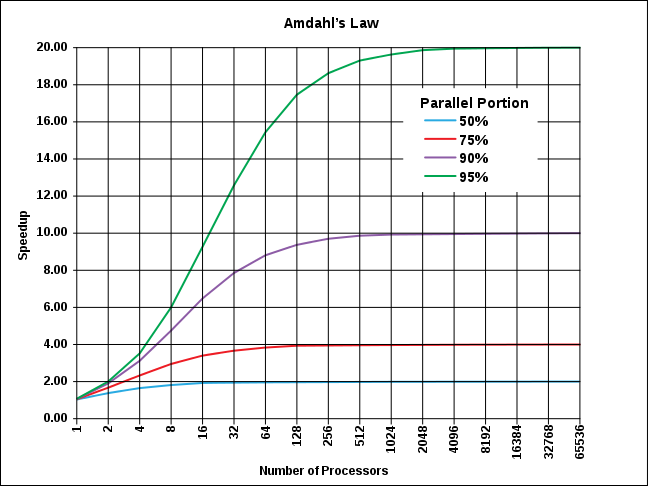
\includegraphics[width=0.75\textwidth]{imgs/AmdahlsLaw.png}}%
\rightline{\tiny http://en.wikipedia.org/wiki/File:AmdahlsLaw.svg}
\smallskip
\end{frame}

\begin{frame}{The Bottom Line}
\begin{itemize}
\item{Parallelisation requires effort:}
\begin{itemize}
\item{There are libraries to help (e.g. \alert{OpenMP}, \alert{MPI}).}
\item{First optimise performance on one CPU, then make $p$ as large as possible.}
\end{itemize}
\pause
\item{The scaling limit: eventually using more CPUs becomes \alert{detrimental} instead of helpful.}
\end{itemize}
\end{frame}

\begin{frame}{Basics: Data Intensive Problems}
\begin{itemize}
\item{Distribute the \alert{data} for a \alert{single problem} across multiple CPUs to reduce the overall execution time.}
\pause
\item{The \emph{same} work may be done on each data segment.}
\pause
\item{Rapid movement of data to and from disk is more important than inter-CPU communication.}
\pause
\item{\alert{Big Data} problems of great current interest -}
\item{Hadoop/MapReduce}
\item{Life Sciences (genomics) and elsewhere.}
\end{itemize}
\end{frame}

\begin{frame}{Basics: High Throughput}
\begin{itemize}
\item{Distribute \alert{independent}, \alert{multiple problems} across multiple CPUs to reduce the overall execution time.}
\pause
\item{Workload is trivially (or \emph{embarrassingly}) parallel:}
\begin{itemize}
\item[$\ast$]{Workload breaks up naturally into \emph{independent} pieces.}
\item[$\ast$]{Each piece is performed by a separate process/thread on a separate CPU (concurrently).}
\item[$\ast$]{\alert{Little or no inter-CPU communication}.}
\end{itemize}
\pause
\item{Emphasis is on throughput over a period, rather than on performance on a single problem.}
\pause
\item{Compute intensive capable $\Rightarrow$ high throughput capable}
\pause
\item{\color{red}Compute intensive capable $\not\Leftarrow$ high throughput capable} 
\end{itemize}
\end{frame}

\begin{frame}{Basics: Memory Intensive Problems}
\begin{itemize}
\item{Require aggregation of large memory into a \alert{single system image} (i.e.\ a single computer running Linux).}
%\pause
%\begin{description}
%\item{\alert{NB Memory (fast, volatile) not disk (slow, non-volatile).}}
%\end{description}
\pause
\item{Technically more challenging to build machines (very fast, low latency interconnection between \alert{all} CPUs and \alert{all} memory).}
\pause
\item{Coding/porting easier (memory appears seamless).}
\pause
\item{Optimisation harder (memory is actually highly nonuniform).}
\pause
\item{Historically, the arena of large \alert{SGI} systems.}
\pause
\item{Nowadays, similar complexity inside single commodity servers.}
\end{itemize}
\end{frame}


\section{Inside a Modern Computer}
\begin{frame}{Basics: Inside a Modern Computer}{CPUs in a box}
\only<1-7>{%
\begin{itemize}
\item<1-7>{Today's commodity servers already aggregate both CPUs and memory to make a single system image in a single box.}
\item<2-7>{Even small computers now have multiple CPU cores per socket\hfill\\
\visible<3-7>{\alert{$\implies{}$each socket is a Symmetric Multi-Processor (SMP).}}}
\item<4-7>{Larger computers have multiple sockets (each with local memory):\hfill\\
{}\qquad all CPU cores (unequally) share the node memory\hfill\\
{}\qquad \visible<5-7>{$\implies{}$the node is a \alert{shared memory} multiprocessor}\\
{}\qquad \visible<6-7>{with Non-Uniform Memory Architecture (\alert{NUMA})}\\
{}\qquad \visible<7>{but users still see a single computer (\alert{single system image}).}}
\end{itemize}
}%
\end{frame}

\begin{frame}{Basics: Inside a Modern Computer}{CPUs in a box}
\centerline{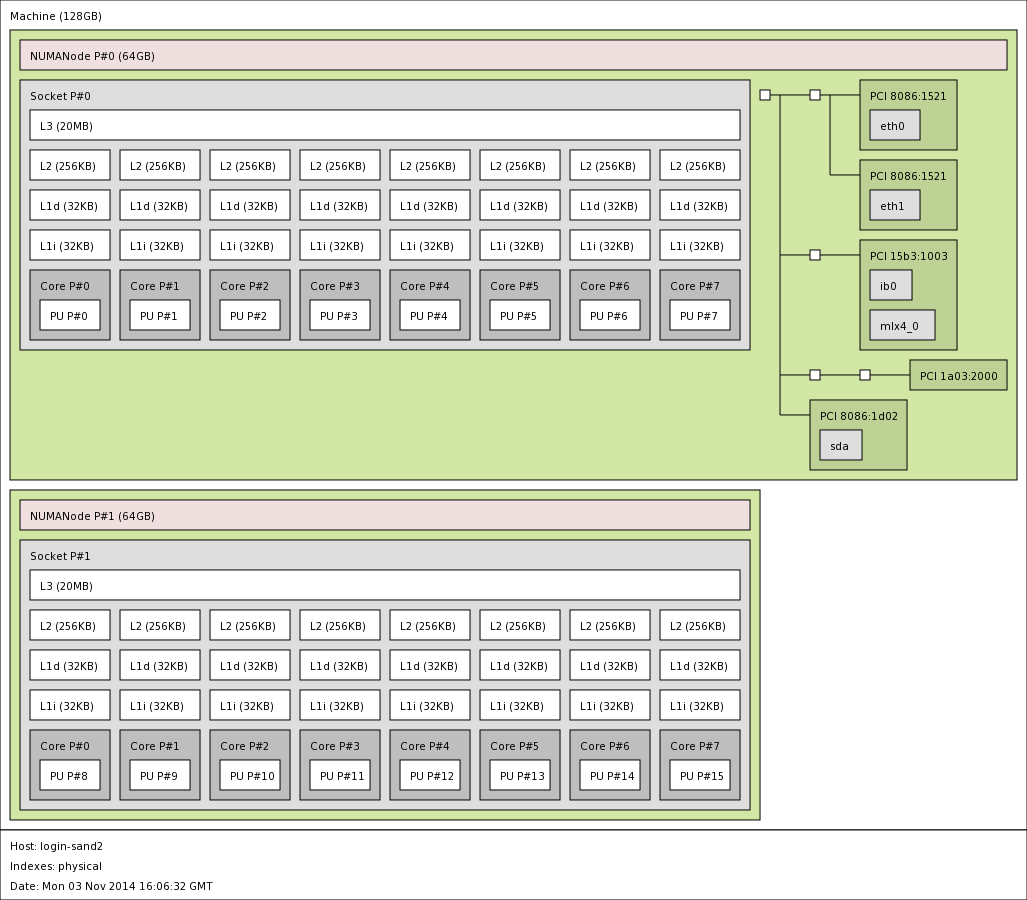
\includegraphics[width=0.8\textwidth]{imgs/lstopo.png}}
\end{frame}

\section{How to Build a Supercomputer}
\begin{frame}{Basics: How to Build a Supercomputer}
\only<1,2>{\begin{itemize}
\item{A supercomputer aggregates contemporary CPUs and memory to obtain increased computing power.}
\pause
\item{Usually today these are \alert{clusters}.}
\end{itemize}}
\only<3->{\begin{enumerate}
\item{Take some (multicore) CPUs plus some memory.}
\begin{itemize}
\item<4->{Could be an off-the-shelf server, or something more special.}
\item<5->{A NUMA, shared memory, multiprocessor building block: a \alert{node}.}
\end{itemize}
\end{enumerate}
}
\end{frame}


\begin{frame}{Basics: How to Build a Supercomputer}
\begin{tabular}{ll}
\parbox[c]{0.5\textwidth}{\begin{enumerate}
\setcounter{enumi}{1}
\item{Connect the nodes with one or more \alert{networks}.}
\pause
\null\par
Faster network for \alert{inter-CPU communication across nodes}.\par
Slower network for \alert{management} and \alert{provisioning}.\par
\alert{Storage} may use either.
\end{enumerate}}
&\vbox to 0pt{\vss\vskip 0.25cm\leftline{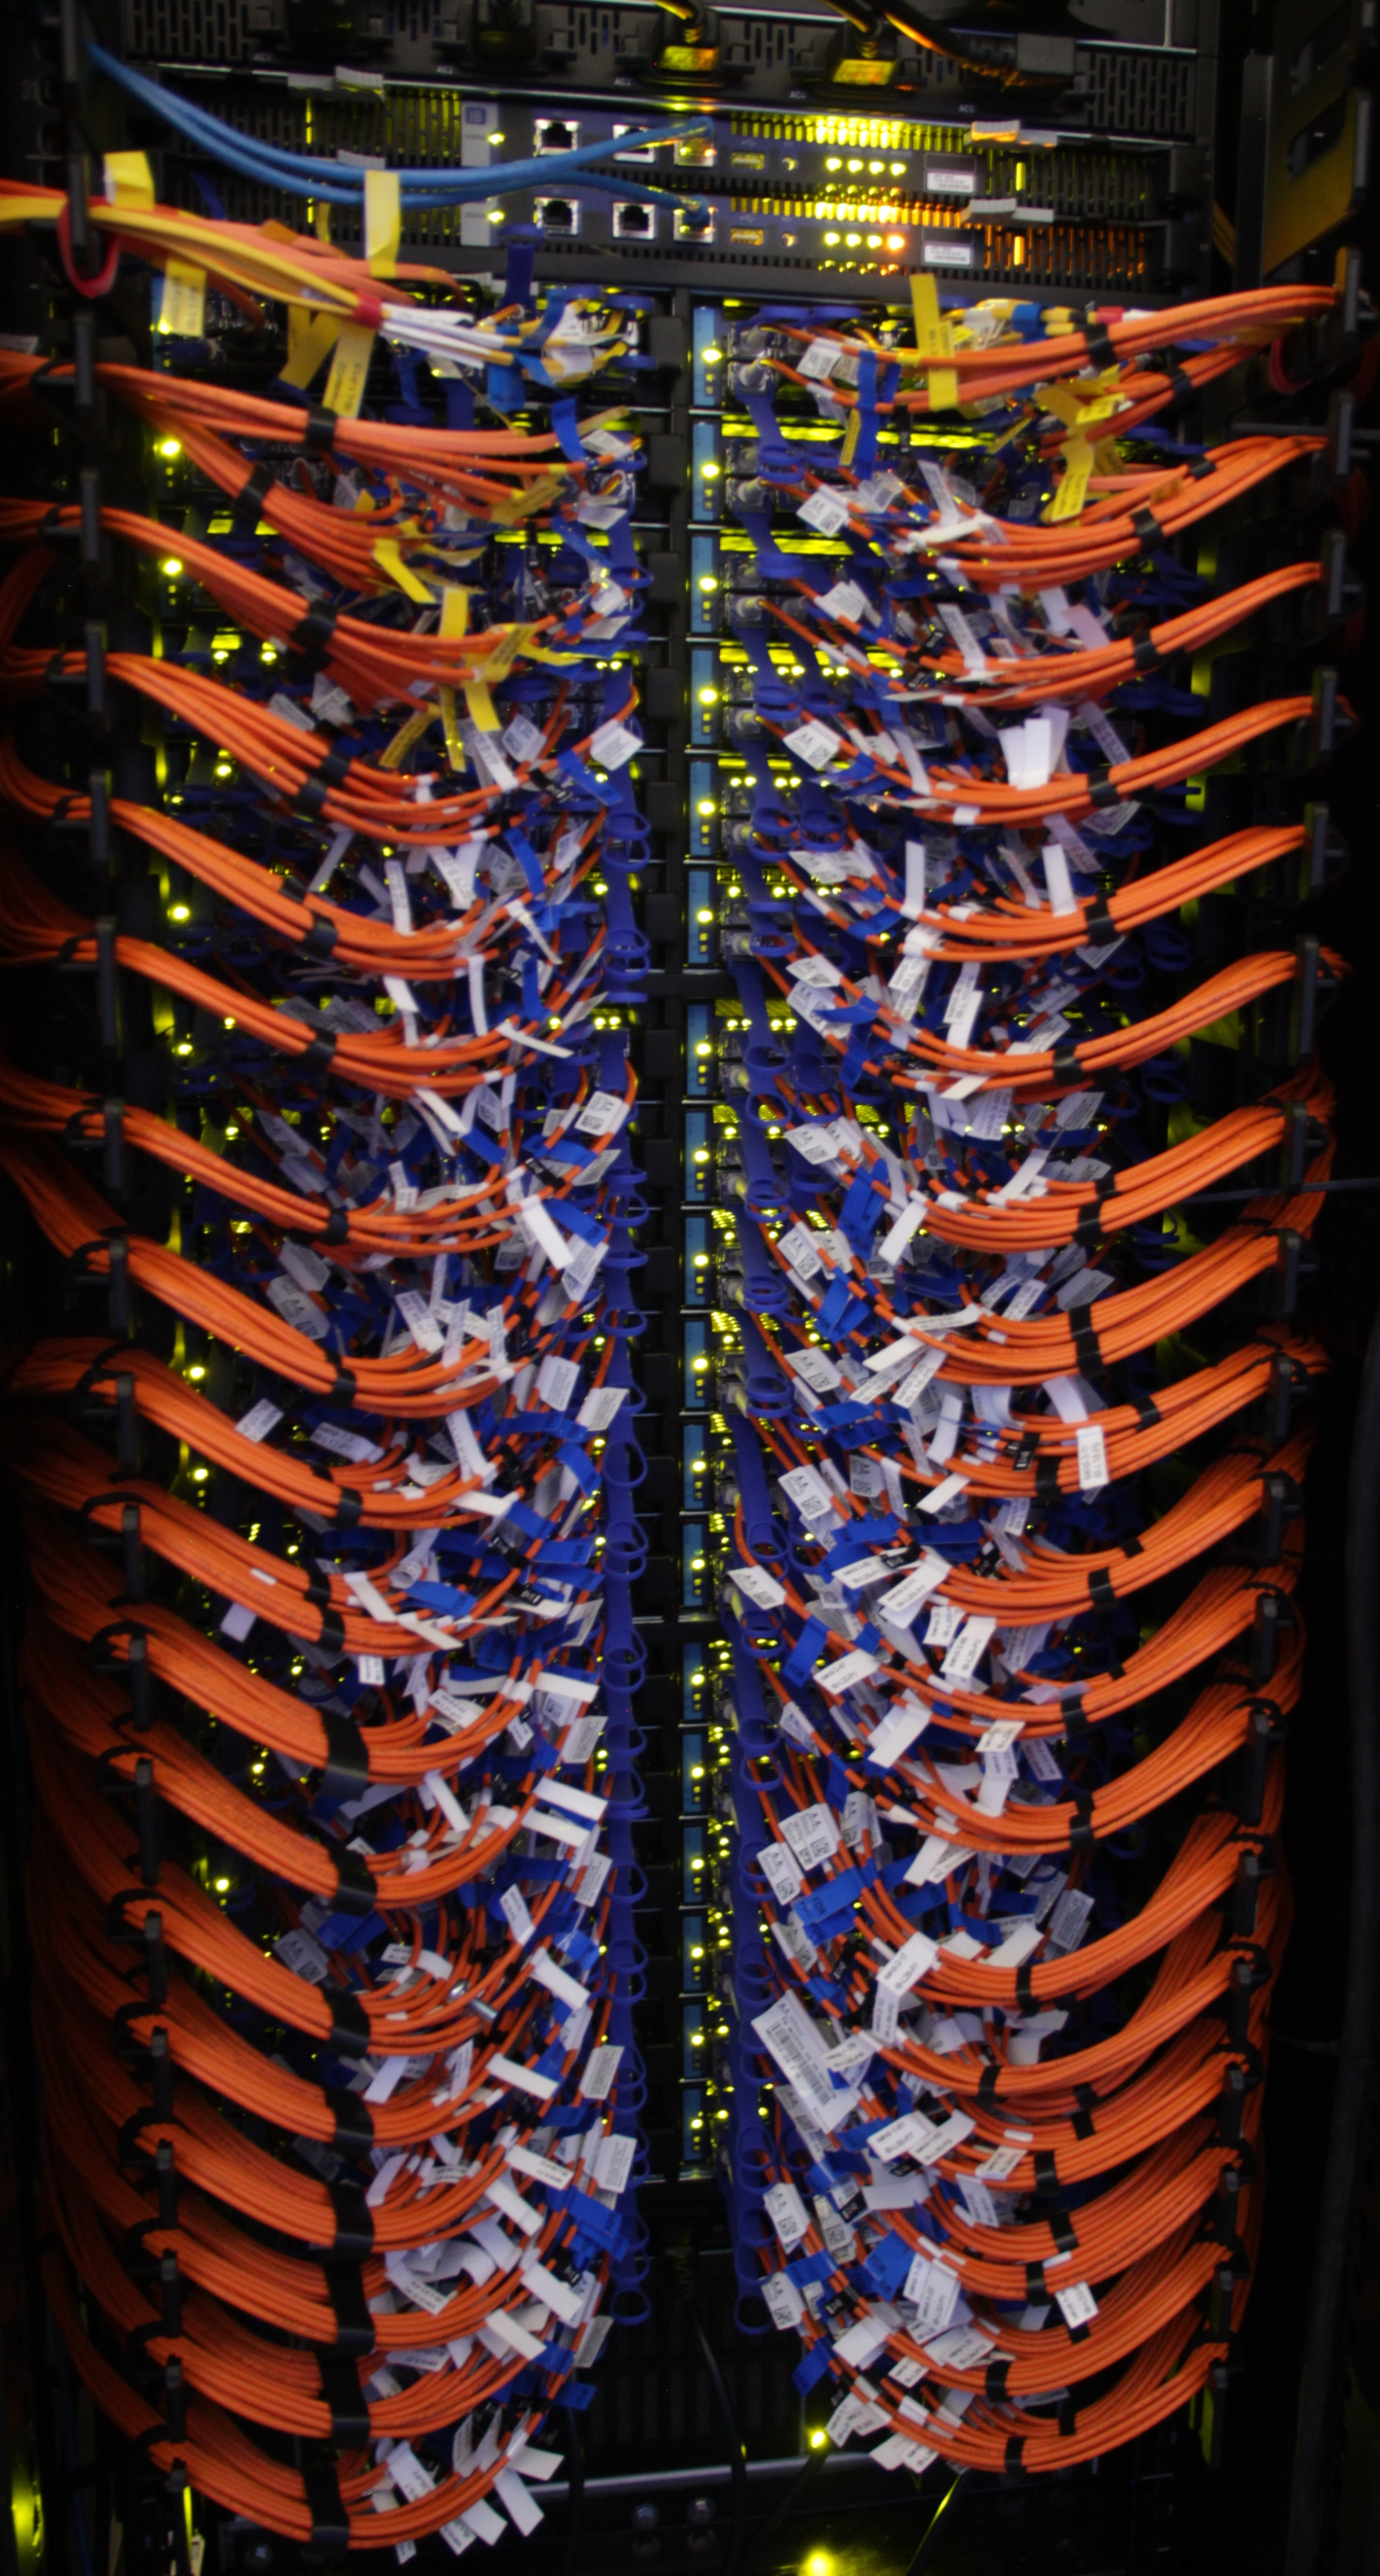
\includegraphics[height=0.85\textheight]{imgs/coreib.jpg}}\vss}\\
\end{tabular}
\end{frame}

\begin{frame}{Basics: How to Build a Supercomputer}
\begin{enumerate}
\setcounter{enumi}{2}
\item{Logically bind the nodes}
\begin{itemize}
\item{Clusters consist of distinct nodes (i.e. separate Linux computers)\hfill\\
on common private network(s) and controlled centrally.}
\begin{itemize}
\item[$\ast$]{Private networks allow CPUs in different nodes to communicate.}
\pause
\item[$\ast$]{Clusters are \alert{distributed memory} machines:\hfill\\
\alert{Each process/thread sees only its local node's CPUs and memory (without help).}}
\pause
\item[$\ast$]{\color{red}Each process/thread must fit within a single node's memory.}
\end{itemize}

%\pause
%\item{More expensive machines logically bind nodes into a single system\hfill\\
%{}\qquad i.e. CPUs \alert{and} memory.}
%\begin{itemize}
%\item[$\ast$]{E.g.\ SGI UV.}
%\item[$\ast$]{Private networks allow CPUs to see CPUs and memory in other nodes.}
%\pause
%\item[$\ast$]{These are \alert{shared memory} machines.}
%\item[$\ast$]{Logically a single system - 1 big node - but very non-uniform.}
%\item[$\ast$]{A single process can span the entire system.}
%\end{itemize}
\end{itemize}
\end{enumerate}

\end{frame}

\section{Programming a Multiprocessor Machine}
\begin{frame}{Basics: Programming a Multiprocessor Machine}
\only<1-3>{\begin{itemize}
\item{Non-parallel (serial) code}
\begin{itemize}
\item[$\ast$]{\alert{For a single node as for a workstation.}}
\pause
\item[$\ast$]{Typically \alert{run as many copies per node as CPUs}, assuming node memory is sufficent.}
\pause
\item[$\ast$]{\alert{Replicate across multiple nodes.}}
\end{itemize}
\end{itemize}}
\only<4->{\begin{itemize}
\item{Parallel code}
\begin{itemize}
\item<5->[$\ast$]{\alert{Shared memory methods within a node.}\hfill\\
E.g. pthreads, OpenMP.}
\item<6->[$\ast$]{\alert{Distributed memory methods spanning multiple nodes.}\hfill\\
Message Passing Interface (MPI).}
\end{itemize}
\end{itemize}}

\end{frame}

\section{Summary}

\begin{frame}{Basics: Summary}

  \begin{itemize}
  \item<1->{\alert{Why have a supercomputer?}}
  \begin{itemize}\item<2->{Big single problems, many problems, Big Data.}\end{itemize}
  \item<3->{Most current supercomputers are \alert{clusters} of separate \alert{nodes}.}
  \item<4->{Each node has \alert{multiple CPUs} and \alert{non-uniform shared memory}.}
  \item<5->{\alert{Parallel} code uses shared memory (\alert{pthreads/OpenMP}) within a node, distributed memory (\alert{MPI}) spanning multiple nodes.}
  \item<6->{\alert{Non-parallel} code uses the memory of one node, but may be copied across many.}
  \end{itemize}
  \end{frame}

